% Stereographic and cylindrical map projections
% Author: Tomasz M. Trzeciak
% Source: LaTeX-Community.org 
%         <http://www.latex-community.org/viewtopic.php?f=4&t=2111>
\documentclass{standalone}
\usepackage{tikz}
\usetikzlibrary{calc,fadings,decorations.pathreplacing, arrows.meta}
%% helper macros

\newcommand\pgfmathsinandcos[3]{%
  \pgfmathsetmacro#1{sin(#3)}%
  \pgfmathsetmacro#2{cos(#3)}%
}
\newcommand\LongitudePlane[3][current plane]{%
  \pgfmathsinandcos\sinEl\cosEl{#2} % elevation
  \pgfmathsinandcos\sint\cost{#3} % azimuth
  \tikzset{#1/.style={cm={\cost,\sint*\sinEl,0,\cosEl,(0,0)}}}
}
\newcommand\LatitudePlane[3][current plane]{%
  \pgfmathsinandcos\sinEl\cosEl{#2} % elevation
  \pgfmathsinandcos\sint\cost{#3} % latitude
  \pgfmathsetmacro\yshift{\cosEl*\sint}
  \tikzset{#1/.style={cm={\cost,0,0,\cost*\sinEl,(0,\yshift)}}} %
}

\newcommand\DrawLongitudeCircle[4][1]{
\LongitudePlane{\angEl}{#2}
\tikzset{current plane/.prefix style={scale=#1}}
% angle of "visibility"
\pgfmathsetmacro\angVis{
atan(sin(#2)*cos(\angEl)/sin(\angEl))} %
\draw[shift={(#3, #4)}][current plane]
(\angVis:1) arc (\angVis:\angVis+180:1);
\draw[shift={(#3, #4)}][current plane,dashed]
(\angVis-180:1)arc(\angVis-180:\angVis:1);
}
\newcommand\DrawLatitudeCircle[4][1]{
\LatitudePlane{\angEl}{#2}
\tikzset{current plane/.prefix style={scale=#1}}
\pgfmathsetmacro\sinVis{
sin(#2)/cos(#2)*sin(\angEl)/cos(\angEl)}
% angle of "visibility"
\pgfmathsetmacro\angVis{
asin(min(1,max(\sinVis,-1)))}
\draw[shift={(#3, #4)}][current plane]
(\angVis:1) arc (\angVis:-\angVis-180:1);
\draw[shift={(#3, #4)}][current plane,dashed]
(180-\angVis:1)arc(180-\angVis:\angVis:1);
}

%% document-wide tikz options and styles

\tikzset{%
  >=latex, % option for nice arrows
  inner sep=0pt,%
  outer sep=2pt,%
  mark coordinate/.style={inner sep=0pt,outer sep=0pt,minimum size=3pt,
    fill=black,circle}%
}

\begin{document}

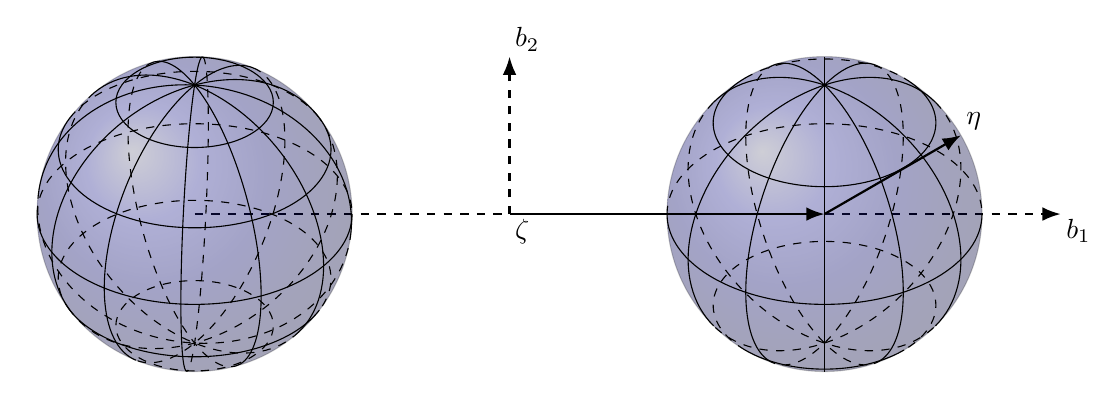
\begin{tikzpicture} % "THE GLOBE" showcase

\def\R{2} % sphere radius
\def\angEl{35} % elevation angle
\def\angAz{-105} % azimuth angle
\def\length{4} % distance from COM to M_1
\def\opacity{0.2}

% centers of the masses
\coordinate (m1) at (\length, 0);
\coordinate (m2) at (-\length, 0);

\draw [ thick, dashed, -Latex] (m2) -- ($ (m1) + (3, 0) $) node [below right] {$b_1$};
\draw [thick, dashed, -Latex] (0, 0) -- (0, \R) node [above right] {$b_2$};
% TODO Make a macro to draw a sphere at a sphefic point
\filldraw[ball color=blue, opacity=\opacity] (m1) circle (\R);
\foreach \t in {-45, 0, 45} { \DrawLatitudeCircle[\R]{\t}{\length}{0} }
\foreach \t in {-30, -60,...,-150} { \DrawLongitudeCircle[\R]{\t}{\length}{0} }

\filldraw[ball color=blue, opacity=\opacity] (m2) circle (\R);
\foreach \t in {-60,-30,...,60} { \DrawLatitudeCircle[\R]{\t}{-\length}{0} }
\foreach \t in {-5,-35,...,-175} { \DrawLongitudeCircle[\R]{\t}{-\length}{0} }

% draw from origin to center of m1
\draw[thick,-Latex] node [below right] {$\zeta$} (0, 0) --  (m1);
\draw[thick,-Latex] (m1) -- ++(30:\R) node [above right] {$\eta$};
\end{tikzpicture}

\end{document} 
